\documentclass[11pt, oneside]{article} 
\usepackage{geometry}
\geometry{letterpaper} 
\usepackage{graphicx}
	
\usepackage{amssymb}
\usepackage{amsmath}
\usepackage{parskip}
\usepackage{color}
\usepackage{hyperref}

\graphicspath{{/Users/telliott/Github/calculus_book/png/}}
% \begin{center} 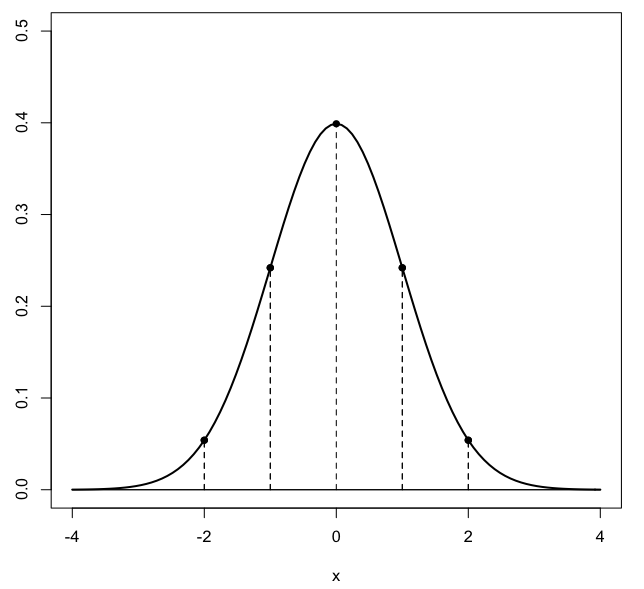
\includegraphics [scale=0.4] {gauss3.png} \end{center}

\title{Natural Numbers}
\date{}

\begin{document}
\maketitle
\Large
\section*{Integers}

The \emph{natural} or counting numbers which everyone learns very early in life are $1, 2, 3$ and so on.

One can get hung up on the question of whether the natural numbers would exist without the problem of counting three sheep or all ten of our fingers.  We will not worry about that.

Mathematicians refer to the \emph{set} of natural numbers and give this set a special symbol, $\mathbb{N}$.  We write
\[ \mathbb{N} = \{ 1, 2, 3 \dots \} \]

The brackets contain between them the \emph{elements} of the set.  The symbol $\in$ means "in the set" or "is a member of the set".

Sometimes people say that
\[ 0 \in \mathbb{N} \]
(0 is a part of the set), but most do not, and we will follow the definition given above.  If you wanted to be explicit about this you could write
\[ 0 \notin \mathbb{N} \]

To construct the set $\mathbb{N}$, start with the smallest element, $1$.  Then add successive elements by forming $a_{n+1} = a_n + 1$.

The dots mean that this sequence of numbers continue forever.  

\subsection*{infinite set}

$\mathbb{N}$ is an infinite set, meaning that there is no largest number in $\mathbb{N}$, no largest $n \in \mathbb{N}$.

Proof:  the proof is by contradiction.  

Suppose $\mathbb{N}$ does have a largest number, $a$.  Well, what about $a + 1$?  By the definition we can construct it, and it is clearly also a member of the set, but $a_{n+1} > a_n$ so $a_n$ is not the largest number in the set.

A second important property of $\mathbb{N}$, as mentioned, is that there is a least number in the set.  If pairwise comparisons are carried out, a single element, the number $1$, has the property that $1 \le n$ for all numbers $n \in \mathbb{N}$.

\subsection*{well-ordered property}

Since we can also find the least member of the set excluding $1$, written $\mathbb{N} \setminus 1$, we can order every number in $\mathbb{N}$.  

This property is called the \textbf{well-ordered} property.

\subsection*{the Integers}

The set $\mathbb{Z}$ contains all the members of $\mathbb{N}$ plus their negatives, as well as the special number $0$, often called the additive identity.

\[ \mathbb{Z} = \{ \dots -2, -1, 0, 1, 2, \dots \} \]

$\mathbb{Z}$ stands for the German word \emph{Zahlen}, Number.  The set $\mathbb{Z}$ are usually referred to as the integers.

$\mathbb{Z}$ is also an infinite set and also has the well-ordered property.  To show this simply order all numbers $p > 0$ with respect to zero using $<$, and all the numbers $n < 0$ using $>$.

\subsection*{inequality}
In the section above we used the symbols $>$ and $<$, greater than and less than, without introducing them.  I'm sure you've seen and used them before.  Among the axioms of the number systems is the collection of \emph{order axioms}.  As an example:

$\circ$ \ $x < y$ means that $y - x$ is positive

$\circ$ \ $y > x$ means that $x < y$

For arbitrary numbers $a$ and $b$ one of three statements is true:  

$a < b$, $a = b$ or $a > b$.

There is no intent to be systematic here.  Let us just mention that these properties (and their kin) are true not just for natural numbers, but also for the rational numbers and the real numbers, which we will talk about soon.  Here are just a few more important theorems in this class:

$\circ$ \ If $a < b$, and $c$ is any number, then $a + c < b + c$

$\circ$ \ If $a < b$, then $-b < -a$

$\circ$ \ If $a < b$ and $c > 0$, then $ac < bc$

\subsection*{sums of integers}

We need to find formulas for several sums.  As a first example, we start with a finite sum, that of the integers from $1$ to $n$:

\[  1 + 2 + 3 + \cdots + n  \]
The numbers we seek are called the triangular numbers.  These are
\[ 1, 3, 6, 10, 15 \cdots \]
Here is a striking "visual proof" of the formula to obtain T$_n$, the $n^{th}$ such number.  The total number of circles in the figure below is $n \times (n+1)$ and this is exactly two times the sum of the integers from $1$ to $n$.

\begin{center} 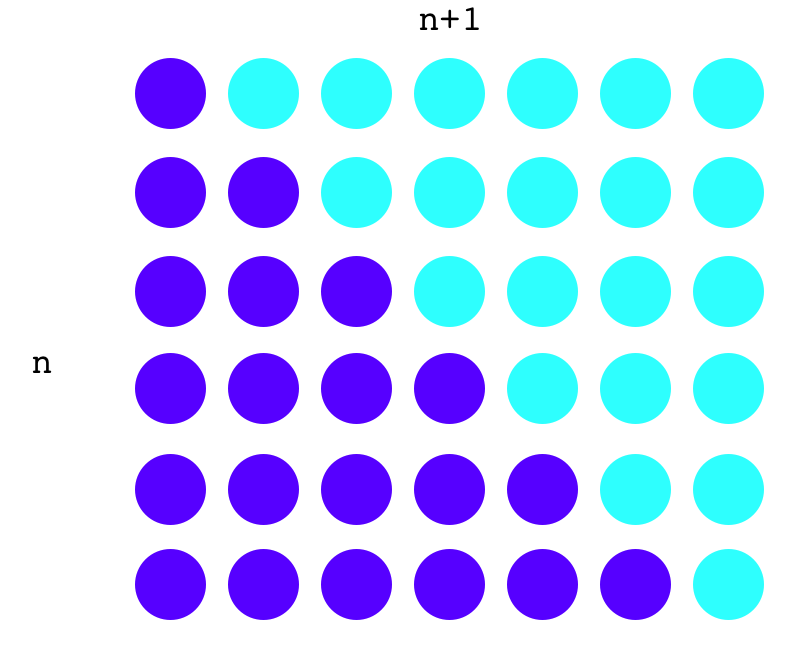
\includegraphics [scale=0.25] {sum_n.png}\end{center}
\[ 2S = n(n+1) \]
There is a famous story about Gauss that, as a schoolboy, he "saw" how to add the integers from $1$ to $100$ as two parallel sums
\[ \ \  1 + \ \ 2 + \ \ 3 + \cdots + 99 + 100 \]
\[ 100 + 99 + 98 + \cdots + 2 + 1 \]
Added together horizontally, these two series must equal twice the sum of $1$ to $100$.  But in the vertical, we notice that we have $n$ sums, each of which is equal to $n+1$.  So, again
\[ 2S = n (n+1) \]
\[ S = \frac{1}{2} \ n (n+1) \]
For $n=100$ the value of the sum is $5050$.  Another way of looking at this result is that between $1$ and $100$ there are $100$ representatives of the "average" value in the sequence, which (because of the monotonic steps) is $(100 + 1)/2 = 50.5$.  

Or alternatively, view the sum as ranging from $0$ to $100$ (with the same answer).  Now there are $101$ examples of the average value ($100 + 0)/2 = 50$).

\subsection*{sum of integer squares}
\begin{center} 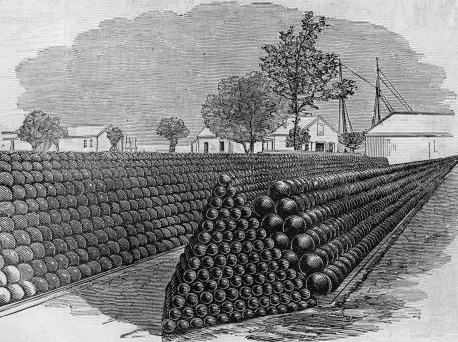
\includegraphics [scale=0.4] {cannonballs.png} \end{center}

Have you ever seen a square stack of marbles, or cannonballs?  The number of elements on each level is the square of a natural number.  We ask, what is the total number:
\[ S = 1^2 + 2^2 + \dots + n^2 = \ ? \]

The answer is not obvious, but we will see how to prove it later using a method called induction.  We will also see how to deduce it.  For now it is enough to give the result:
\[ S = \frac{1}{3} \cdot n \cdot (n + \frac{1}{2}) \cdot (n + 1) \]
which is sometimes given as
\[ S = \frac{n(n+1)(2n+1)}{6} \]

Given the formula for the volume of a cone or pyramid, the factor $1/3$ is not surprising.


\end{document}